\documentclass[12pt,a4paper]{article}
\usepackage{amsmath}
\usepackage{amsfonts}
\usepackage{amssymb}
\usepackage{graphicx}
\usepackage{secdot}
\usepackage[left=2cm,right=2cm,top=2cm,bottom=2cm]{geometry}

\author{ Shibayan Biswas, AE21B109\\ Department of Aerospace Engineering\\ IIT Madras\\[3ex] Instructor:\\ \large Professor Dr. Manikandan Mathur}

\title{Experiment- 2}

\date{September 12, 2022}

\begin{document}

\maketitle

\hline

\section{Aim:}
Verifying linear variation of hydro-static pressure with height of the water level and verification of the center of pressure.
\section{Introduction:}
Hydro-static forces are the resultant force caused by the pressure loading of a liquid acting on submerged surfaces. Calculation of the hydro-static force and the location of the center of pressure are fundamental subjects in fluid mechanics. The center of pressure is a point on the immersed surface at which the resultant hydro-static pressure force acts.
\section{Practical Application:}
The location and magnitude of water pressure force acting on water-control structures, such as dams, levees, and gates, are very important to their structural design. Hydro-static force and its line of action is also required for the design of many parts of hydraulic equipment.
\section{Objective:}
The objectives of this experiment are the following:
\begin{itemize}
\item To determine the hydro-static force due to water acting on a partially or fully submerged surface.
\item To determine, both experimentally and theoretically, the center of pressure.
\end{itemize}
\section{Method:}
In this experiment, the hydro-static force and center of pressure acting on a vertical surface will be determined by increasing the water depth in the apparatus water tank and by reaching an equilibrium condition between the moments acting on the balance arm of the test apparatus. The forces which create these moments are the weight applied to the balance arm and the hydro-static force on the vertical surface.
\section{Equipment:}
Equipment required to carry out this experiment is the following:
\begin{itemize}
\item Arm-field F1-12 Hydro-static Pressure Apparatus
\item A jug
\item Calipers or rulers for measuring the actual dimensions of the quadrant
\end{itemize}
\section{Experiment Description:}
\\The equipment is comprised of a rectangular transparent water tank, a fabricated quadrant, a balance arm, an adjustable counter-balance weight, and a water-level measuring device (Figure 1.1).
\\The water tank has a drain valve at one end and three adjustable screwed-in feet on its base for leveling the apparatus. The quadrant is mounted on a balance arm that pivots on knife edges. The knife edges coincide with the center of the arc of the quadrant; therefore, the only hydro-static force acting on the vertical surface of the quadrant creates moment about the pivot point. This moment can be counterbalanced by adding weight to the weight hanger, which is located at the left end of the balance arm, at a fixed distance from the pivot. Since the line of actions of hydro-static forces applied on the curved surfaces passes through the pivot point, the forces have no effect on the moment. The hydro-static force and its line of action (center of pressure) can be determined for different water depths, with the quadrant’s vertical face either partially or fully submerged.\\
\\A level indicator attached to the side of the tank shows when the balance arm is horizontal. Water is admitted to the top of the tank by a flexible tube and may be drained through a cock in the side of the tank. The water level is indicated on a scale on the side of the quadrant.\\
\clearpage
\begin{figure}[!ht]
	\begin{center}
		\framebox{
			\includegraphics[scale=0.8]{Hydrostatic_Pressure_Apparatus.png}
		}
	\end{center}
	\caption{Armfield F1-12 Hydrostatic Pressure Apparatus}
	\label{Armfield F1-12 Hydrostatic Pressure Apparatus}
\end{figure}
\section{Theory:}
In this experiment, when the quadrant is immersed by adding water to the tank, the hydro-static force applied to the vertical surface of the quadrant can be determined by considering the following:
\begin{itemize}
\item The hydro-static force at any point on the curved surfaces is normal to the surface and resolves through the pivot point because it is located at the origin of the radii. Hydrostatic forces on the upper and lower curved surfaces, therefore, have no net effect – no torque to affect the equilibrium of the assembly because the forces pass through the pivot.
\item The forces on the sides of the quadrant are horizontal and cancel each other out (equal and opposite).
\item The hydro-static force on the vertical submerged face is counteracted by the balance weight. The resultant hydro-static force on the face can, therefore, be calculated from the value of the balance weight and the depth of the water.
\item The system is in equilibrium if the moments generated about the pivot points by the hydro-static force and added weight (=mg) are equal, that is:
\begin{equation}
	\text{mg} \times \text{L} = \text{F} \times \text{y}
\end{equation}
m : Mass on the weight hanger\\
L : Length of the balance arm (Figure 1.2)\\
F : Hydrostatic force\\
y : Distance between the pivot and the center of pressure (Figure 1.2).\\
\\Then, calculated hydro-static force and center of pressure on the vertical face of the quadrant can be compared with the experimental results.\\
\end{itemize}
\subsection{Hydrostatic Force:}
The magnitude of the resultant hydro-static force (F) applied to an immersed surface is given by:
\begin{equation}
	\text{F} = \text{$P_c$A} = \text{$\rho$g$y_c$A}
\end{equation}
$P_c$ : pressure at centroid of the immersed surface\\
A: area of the immersed surface\\
$y_c$ : centroid of the immersed surface measured from the water surface\\
$\rho$ : density of fluid\\
g : acceleration due to gravity\\
\\The hydro-static force acting on the vertical face of the quadrant can be calculated as:
\begin{itemize}
\item Partially immersed vertical plane:
\begin{equation}
	\text{F} = \frac{1}{2} \text{$\rho gBd^2$}
\end{equation}
\item Fully immersed vertical plane:
\begin{equation}
	\text{F} = \text{$\rho gBD(d - \frac{D}{2})$}
\end{equation}
B : width of the quadrant face\\
d : depth of water from the base of the quadrant\\
D : height of the quadrant face\\
\end{itemize}
\subsection{Theoretical determination of Center of Pressure:}
The center of pressure  is calculated as:
\begin{equation}
	\text{$y_p$} = \frac{\text{$I_x$}}{\text{A$y_c$}}
\end{equation}
$I_x$ is the $2^{nd}$ moment of area of immersed body about an axis in the free surface. By use of the parallel axes theorem:
\begin{equation}
	\text{$I_x$} = \text{$I_c$} + \text{A$y_c^2$}
\end{equation}
where $y_c$ is the depth of the centroid of the immersed surface, and $I_c$ is the $2^{nd}$ moment of area of immersed body about the centroidal axis. $I_x$  is calculated as:
\begin{itemize}
\item Partially immersed vertical plane:
\begin{equation}
	\text{$I_x$} = \frac{Bd^3}{12} + \text{Bd$(\frac{d}{2})^2$} = \frac{Bd^3}{3}
\end{equation}
\item Fully immersed vertical plane:
\begin{equation}
	\text{$I_x$} = \text{BD[$\frac{D^2}{12}$ + (d - $\frac{D}{2})^2$)]}
\end{equation}
\end{itemize}
The depth of the center of pressure below the pivot point is given by:
\begin{equation}
	\text{$y$} = \text{$y_p$} + \text{H} - \text{d}
\end{equation}
in which H is the vertical distance between the pivot and the base of the quadrant. Substitution of Equation (8) and into (5) and then into (9) yields the theoretical results, as follows:
\begin{itemize}
\item Partially immersed vertical plane:
\begin{equation}
	\text{y} = \text{H} - \frac{d}{3}
\end{equation}
\item Fully immersed vertical rectangular plane:
\begin{equation}
	\text{y} = \frac{\text{$\frac{D^2}{12}$ + (d - $\frac{D}{2})^2$)}}{\text{d - $\frac{D}{2}$}} + \text{H} - \text{d} 
\end{equation}
\end{itemize}
\begin{figure}[!ht]
	\begin{center}
		\framebox{
			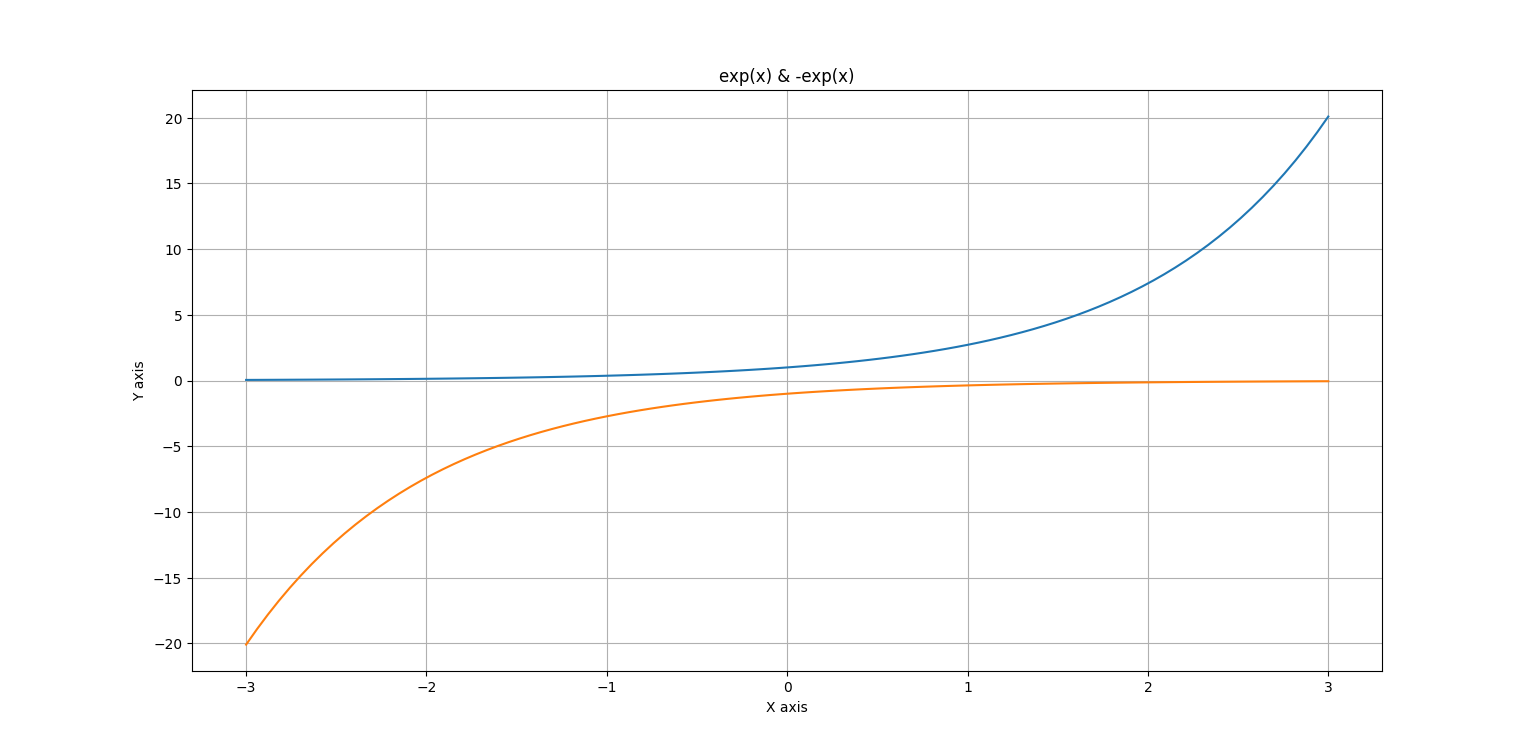
\includegraphics[scale=0.35]{Figure_1.png}
		}
	\end{center}
	\caption{Partially submerged quadrant (c: centroid, p: center of pressure)}
	\label{Partially submerged quadrant (c: centroid, p: center of pressure)}
\end{figure}
\clearpage
\begin{figure}[!ht]
	\begin{center}
		\framebox{
			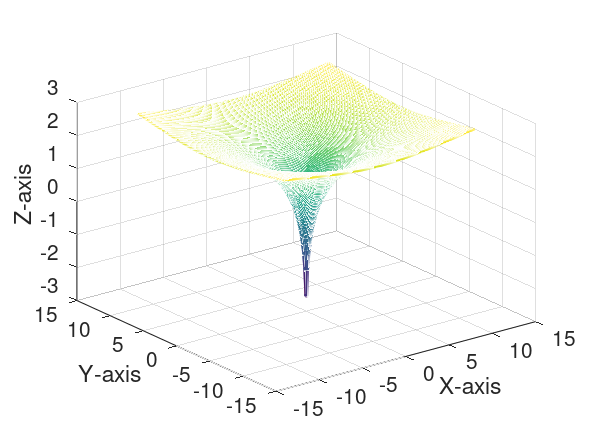
\includegraphics[scale=0.35]{Figure_2.png}
		}
	\end{center}
	\caption{Fully submerged quadrant (c: centroid, p: center of pressure)}
	\label{Fully submerged quadrant (c: centroid, p: center of pressure)}
\end{figure}
\subsection{Experimental determination of Center of Pressure:}
For equilibrium of the experimental apparatus, moments about the pivot are given by Equation (1). By substitution of the derived hydro-static force, F from Equation (3 and 4), we have:
\begin{itemize}
\item Partially immersed vertical plane:
\begin{equation}
	\text{y} = \frac{\text{mgL}}{\text{F}} = \frac{\text{2mL}}{\text{\rho $Bd^2$}}
\end{equation}
\item Fully immersed vertical rectangular plane:
\begin{equation}
	\text{y} = \frac{\text{mL}}{\text{$\rho BD(d - \frac{D}{2})$}} 
\end{equation}
\end{itemize}
\section{Experimental Procedure:}
Begin the experiment by measuring the dimensions of the quadrant vertical end-face (B and D) and the distances (H and L), and then perform the experiment by taking the following steps:
\begin{itemize}
\item Wipe the quadrant with a wet rag to remove surface tension and prevent air bubbles from forming.
\item Place the apparatus on a level surface, and adjust the screwed-in feet until the built-in circular spirit level indicates that the base is horizontal. (The bubble should appear in the center of the spirit level.)
\item Position the balance arm on the knife edges and check that the arm swings freely.
\item Place the weight hanger on the end of the balance arm and level the arm, using the counter weight, so that the balance arm is horizontal.
\item Add 50 grams to the weight hanger.
\item Add water to the tank and allow time for the water to settle.
\item Close the drain valve at the end of the tank, then slowly add water until the hydro-static force on the end surface of the quadrant is balanced. This can be judged by aligning the base of the balance arm with the top or bottom of the central marking on the balance rest.
\item Record the water height, which displayed on the side of the quadrant in mm. If the quadrant is partially submerged, record the reading in the partially submerged portion of the Raw Data Table.
\item Repeat the steps, adding 50 g weight each time, until the final weight of 500 g is reached. When the quadrant is fully submerged, record the readings in the fully submerged part of the Raw Data Table.
\item Repeat the procedure in reverse by progressively removing the weights.
\item Release the water valve, remove the weights, and clean up any spilled water.
\end{itemize}
\section{Results:}
The tables representing the experimental and the theoretical values along with the plots showing the variation of the respective values for the following experiment is provided in this section:
\begin{table}[h]
\begin{center}
\begin{tabular}{|c|c|c|}
\hline
Serial No. & Mass, m(kg) & Depth of Immersion, d(m) \\
\hline
1 & 0.35 & 0.131  \\
2 & 0.30 & 0.120  \\
3 & 0.25 & 0.106  \\
\hline
\end{tabular}
\caption{Raw Data Table for Partially Immersed Condition}
\label{tab:progs}
\end{center}
\end{table}
\begin{table}[h]
\begin{center}
\begin{tabular}{|c|c|c|}
\hline
Serial No. & Mass, m(kg) & Depth of Immersion, d(m) \\
\hline
1 & 0.20 & 0.094 \\
2 & 0.17 & 0.086 \\
3 & 0.14 & 0.078\\
\hline
\end{tabular}
\caption{Raw Data Table for Completely Immersed Condition}
\label{tab:progs}
\end{center}
\end{table}
\clearpage
\begin{table}
\begin{center}
\begin{tabular}{|p{2cm}|p{2cm}|p{2cm}|p{2cm}|p{2.5cm}|p{2.5cm}|p{2.5cm}|}
\hline
Mass(kg) & Height(m) & Moment ($M_w$) & Force(N) & Experimental ($y_p$) & Experimental ($\Delta$$y_p$) & Theoretical ($\Delta$$y_p$) \\ 
\hline
0.35&0.131&0.994&5.960&0.158&0.008&0.010\\
0.30&0.120&0.809&5.150&0.157&0.007&0.012\\
0.25&0.106&0.674&4.120&0.164&0.014&0.015\\
0.20&0.094&0.540&3.251&0.166&0.013&0.017\\
0.17&0.086&0.459&2.721&0.169&0.012&0.014\\
0.14&0.078&0.378&2.238&0.169&0.008&0.013\\
\hline
\end{tabular}
\caption{Result Table}
\label{Result Table}
\end{center}
\end{table}
\begin{figure}[!ht]
	\begin{center}
			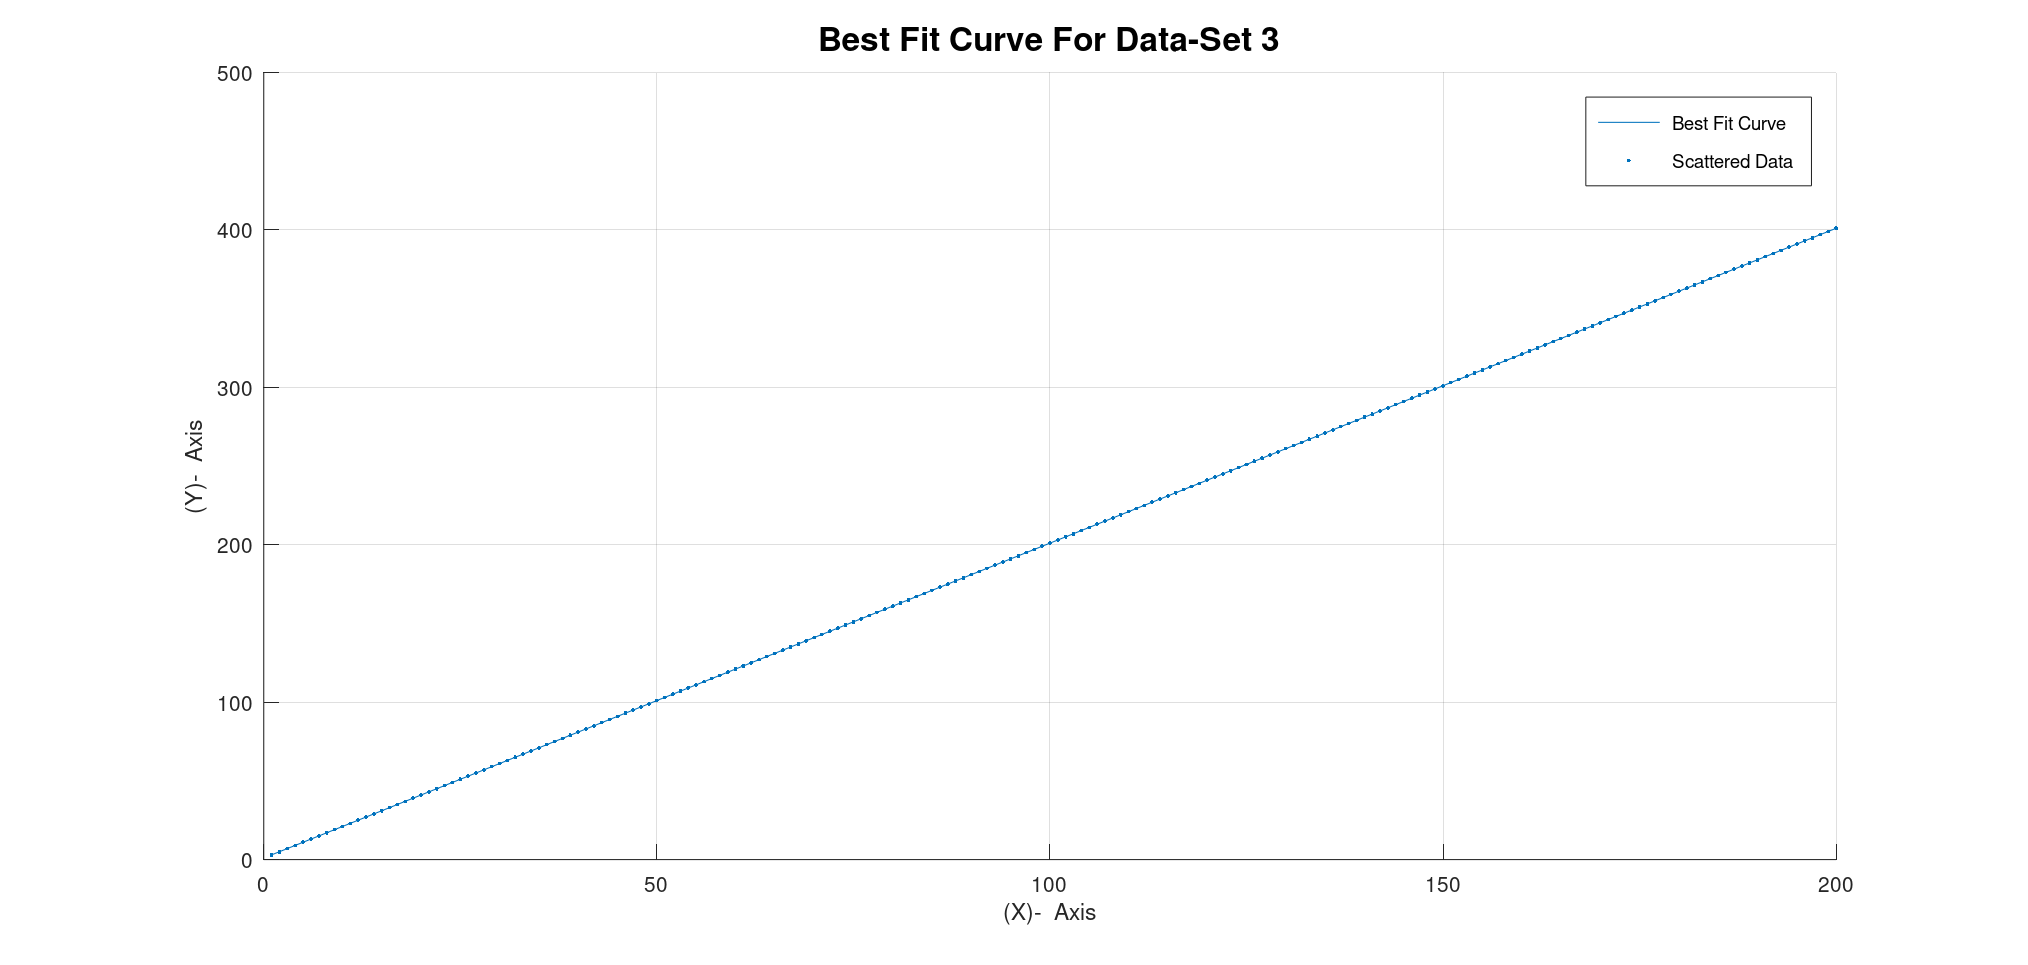
\includegraphics[scale=0.95]{Figure_5.png}
	\end{center}
	\caption{$\Delta$$y_p$ v/s Height(h)}
	\label{$\Delta$$y_p$ v/s Height(h)}
\end{figure}
\section{Sources of Error:}
While in general the results seem to be in line with what is expected, there is still the possibility
of error. This may be due to a variety of mistakes in the experiment. For example, there is the possibility of human error in reading when the balance bridge arm is level. This would lead to an inaccurate water height reading, which would consequently affect everything height was used to calculate. There may also have been human error in reading the height of the water in the chamber: also affecting the height measurement and all subsequent calculations.\\
Experimentally, a source of error may be in the possibility of water splashing onto the balance bridge arm while it was poured. This would cause an artificial increase in weight beyond the weight due to the applied masses. As a result, the hydro-static force to counteract the masses moment would also be artificially high, and an artificially high water height would be read off the pressure system. Finally, the applied masses were not weighed prior to their application onto the balance bridge arm. Thus, the applied mass may weigh more due to accumulation of oils from being handled. As a result, an artificially high mass would be recorded, resulting in what appears to be a water height that it too high. However, these errors are so minor that it
is likely that, even if they were present in the experiment, they would have little, to no, effect on the results.
\section{Conclusion:}
The Edibon Hydro-statics Pressure System accurately measures the height of the water in the chamber needed to calculate both hydrostatic force acting on the vertical rectangular quadrant and the center of pressure at which this force acts, with a low standard deviation from the theoretical water height for both partially and fully submerged surfaces. This is confirmed by the linear plots of theoretical versus measured water height in which the slope is approximately one for both the partially and fully submerged surfaces. The data gathered from the pressure system also supports the relationships between variables as they are presented in the equations given to calculate hydrostatic force, center of pressure, and mass. In other words, the hydro-static force acting on both partially and fully submerged vertical rectangular surface increases
as the height of the fluid (water) in the chamber increases. This relationship is supported by the plots of mass versus theoretical height when the balance of the moments about the pivot is considered. For both partially and fully submerged surfaces, the center of pressure (measured from the balance bridge arm down) decreases towards the centroid of the quadrant as the height of water in the chamber increases.
\end{document}